\section{YLABEL Plot Y-axis Label Function}

\subsection{Usage}

This command adds a label to the y-axis of the plot.  The general syntax
for its use is
\begin{verbatim}
  ylabel('label')
\end{verbatim}
or in the alternate form
\begin{verbatim}
  ylabel 'label'
\end{verbatim}
or simply
\begin{verbatim}
  ylabel label
\end{verbatim}
You can also specify properties for that label using the syntax
\begin{verbatim}
  ylabel('label',properties...) 
\end{verbatim}
\subsection{Example}

Here is an example of a simple plot with a label on the \verb|y|-axis.
\begin{verbatim}
--> x = linspace(-1,1);
--> y = cos(2*pi*x);
--> plot(x,y,'r-');
--> ylabel('cost');
\end{verbatim}
which results in the following plot.


\centerline{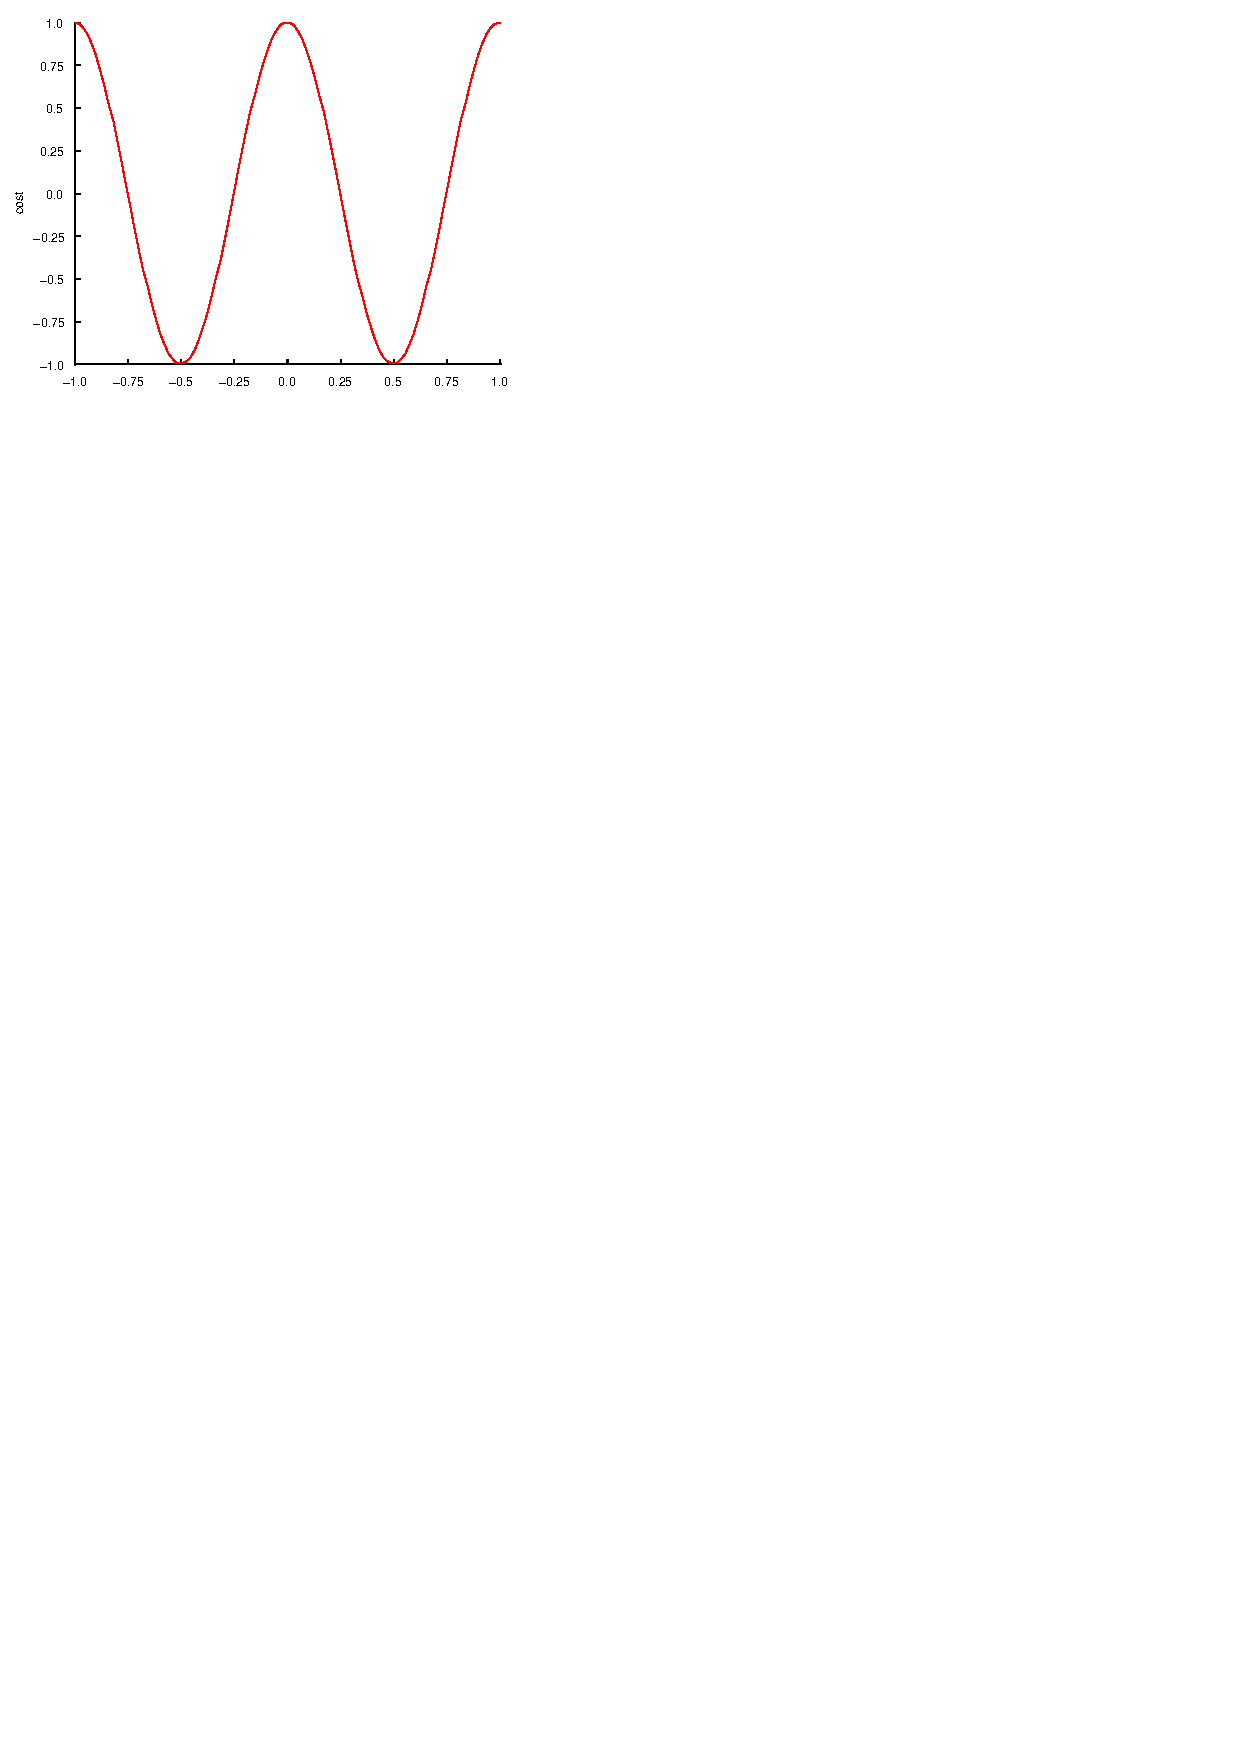
\includegraphics[width=8cm]{ylabel1}}

